
\documentclass[11pt,a4paper,UTF8]{book}

\usepackage[T1]{fontenc}
\usepackage[utf8]{inputenc}
\usepackage{authblk}

\usepackage{fontspec}                  %引入字体设置宏包
\setmainfont{Times New Roman}             %设置英文正文字体
% Courier New
% Book Antique
\setsansfont{Arial}                    %英文无衬线字体
\setmonofont{Courier New}              %英文等宽字体

\usepackage{ctex} %导入中文包
%\usepackage{ulem}
\usepackage{tocvsec2}
\usepackage{verbatim}

\usepackage{tabularx}
\usepackage{longtable}
\usepackage{booktabs} 
\usepackage{multirow}
\usepackage{bbding}
\usepackage{float}
\usepackage{xspace}
\usepackage[none]{hyphenat}

\usepackage{graphicx}
\usepackage{subfigure}
\usepackage{pifont}

\usepackage{hyperref}  %制作pdf的目录
\usepackage{subfiles} %使用多文件方式进行

\usepackage{geometry} %设置页边距的包
\geometry{left=2.5cm,right=2cm,top=2.54cm,bottom=2.54cm} %设置书籍的页边距

\usepackage{url}
\hypersetup{hidelinks, %去红框
	colorlinks=true,
	allcolors=black,
	pdfstartview=Fit,
	breaklinks=true
}

% 调整itemlist中的行间距
\usepackage{enumitem}
\setenumerate[1]{itemsep=0pt,partopsep=0pt,parsep=\parskip,topsep=5pt}
\setitemize[1]{itemsep=0pt,partopsep=0pt,parsep=\parskip,topsep=5pt}
\setdescription{itemsep=0pt,partopsep=0pt,parsep=\parskip,topsep=5pt}

% 超链接样式设置
\usepackage{hyperref}
\hypersetup{
	colorlinks=true,
	linkcolor=blue,
	filecolor=blue,
	urlcolor=blue,
	citecolor=cyan,
}

\usepackage{indentfirst}

\usepackage{listings}
\usepackage[usenames,dvipsnames,svgnames, x11names]{xcolor}

\usepackage[most]{tcolorbox}
\tcbuselibrary{breakable} % 引入 breakable 库
\tcbuselibrary{skins} % 引入 skins 库

%展示代码
\definecolor{mygreen}{rgb}{0,0.6,0}
\definecolor{mygray}{rgb}{0.5,0.5,0.5}
\definecolor{mymauve}{rgb}{0.58,0,0.82}
\definecolor{keywordcolor}{rgb}{0.8,0.1,0.5}
\definecolor{webgreen}{rgb}{0,.5,0}
\definecolor{bgcolor}{rgb}{0.92,0.92,0.92}

%定义CMake
\lstdefinelanguage{CMake}
{morekeywords={
		cmake\_minimum\_required,
		project,
		add\_executable,
		add\_library,
		target\_link\_libraries,
		cmake\_parse\_arguments,
		cmake\_language,
		set, unset,
		option,
		string,
		list,
		math,
		message,
		if, elseif, else, endif,
		mark\_as\_advanced,
		foreach, endforeach,
		while, endwhile,
		add\_subdirectory, include, return, include\_gurad,
		function, endfunction,
		macro, endmacro,
		find\_package,
		cmake\_push\_check\_state,
		cmake\_pop\_check\_state,
		cmake\_reset\_check\_state,
		add\_test,
		set\_tests\_properties, 
		check\_c\_source\_runs,
		check\_cxx\_source\_runs,
		check\_fortran\_source\_runs,
		check\_source\_runs,
		check\_compiler\_flag,
		check\_c\_compiler\_flag,
		check\_cxx\_compiler\_flag,
		check\_fortran\_compiler\_flag,
		check\_symbol\_exists,
		check\_cxx\_symbol\_exists,
		check\_linker\_flag,
		cmake\_policy,
		set\_property,
		get\_property,
		define\_property,
		get\_cmake\_property,
		set\_cmake\_property,
		set\_target\_properties,
		get\_target\_property,
		set\_directory\_properties,
		get\_directory\_property,
		set\_source\_files\_properties,
		get\_source\_file\_property,
		set\_tests\_properties,
		get\_tests\_property,
		get\_test\_property,
		cmake\_print\_properties,
		cmake\_print\_variables,
		variable\_watch,
		include\_guard,
		target\_link\_options,
		target\_compile\_definitions,
		target\_compile\_options,
		include\_directories,
		add\_definitions,
		remove\_definitions,
		add\_compile\_definitions,
		add\_compile\_options,
		link\_libraries,
		link\_directories,
		add\_link\_options,
		target\_include\_directories,
		target\_compile\_features,
		add\_custom\_command,
		add\_custom\_target,
		execute\_process,
		cmake\_path,
		get\_filename\_component,
		file,
		configure\_file,
		generate\_export\_header,
		export,
		find\_file,
		find\_library,
		find\_package,
		find\_program,
		pkg\_check\_modules,
		pkg\_search\_module,
		pkg\_get\_variable,
		add\_test,
		enable\_testing,
		set\_tests\_properties,
		site\_name,
		ctest\_empty\_binary\_directory,
		ctest\_start,
		ctest\_configure,
		ctest\_submit,
		ctest\_build,
		ctest\_memcheck,
		ctest\_upload,
		ctest\_test,
		gtest\_add\_tests,
		gtest\_discover\_tests,
		install,
		write\_basic\_package\_version\_file,
		configure\_package\_config\_file,
		cpack\_add\_component,
		cpack\_add\_install\_type,
		cpack\_add\_component\_group,
		ExternalProject\_Add,
		ExternalProject\_Add\_StepDependencies,
		ExternalProject\_Get\_Property,
		ExternalProject\_Add\_Step,
		FetchContent\_Declare,
		FetchContent\_GetProperties,
		FetchContent\_Populate,
		source\_group,
		target\_precompile\_headers,
		qt5\_wrap\_cpp,
		qt5\_wrap\_ui,
		qt5\_add\_resources,
		qt5\_add\_big\_resources,
		qt5\_add\_binary\_resources,
		qt5\_add\_translation,
		qt5\_create\_translation,
		compile\_definitions,
		add\_llvm\_component\_library,
		add\_llvm\_tool,
		llvm\_multisource,
		llvm\_test\_data,
		doxygen\_add\_docs,
		cmake\_dependent\_option,
		target\_sources,
		conan\_cmake\_autodetect,
		conan\_cmake\_configure,
		conan\_cmake\_install,
		doxygen\_add\_docs,
		check\_source\_compiles,
		check\_language,
		enable\_language,
		add\_dependencies,
		find\_path,
		find\_package\_handle\_standard\_args,
	}, %定义关键字
	sensitive=false, %是否大小写敏感
	morecomment=[l]{\#},
	morestring=[b]",
	morestring=[d]',
}

\lstdefinestyle{styleCXX}{
	language = C++,  
	backgroundcolor=\color{blue!3!white}, 
	%basicstyle = \footnotesize,  
	basicstyle      =   \zihao{-5}\ttfamily,
	numberstyle     =   \zihao{-5}\ttfamily,   
	%breakatwhitespace = false,    
	basewidth       =   0.5em,    
	breaklines = true,                 
	captionpos = b,                    
	commentstyle = \color{mygray}\bfseries,
	%extendedchars = false,             
	frame =shadowbox, 
	framerule=0.5pt,
	%frameround = fttt,
	keepspaces=true,
	keywordstyle=\color{blue}\bfseries, % keyword style
	otherkeywords={string}, 
	numbers=left, 
	numbersep=5pt,
	numberstyle=\tiny\color{mygray},
	rulecolor=\color{black},         
	%showspaces=false,  
	%showstringspaces=false, 
	%showtabs=false,    
	%stepnumber=1,         
	stringstyle=\color{mymauve},        % string literal style
	tabsize=2,          
	columns         =   fixed,
	flexiblecolumns,                   
}


\lstdefinestyle{styleCMake}{
	language=CMake,
	backgroundcolor=\color{blue!3!white}, 
	basicstyle=\tt, 
	breakatwhitespace = false,
	breaklines = true,
	captionpos = b,
	commentstyle = \color{mygray}\bfseries, 
	extendedchars =false,             
	frame=shadowbox, 
	tabsize=2,
	framerule=0.5pt,
	keepspaces=true,
	keywordstyle=\color{blue}\bfseries, % keyword style
	otherkeywords={string}, 
	rulecolor=\color{black},
	showspaces=false,
	showstringspaces=false,
	showtabs=false,
	stepnumber=1,
	stringstyle=\color{purple},        % string literal style
}

\lstdefinestyle{stylePython}{
	language        =   Python, % 语言选Python
	backgroundcolor=\color{blue!3!white}, 
	basicstyle      =   \zihao{-5}\ttfamily,
	numberstyle     =   \zihao{-5}\ttfamily,
	keywordstyle    =   \color{blue},
	keywordstyle    =   [2] \color{teal},
	stringstyle     =   \color{magenta},
	commentstyle    =   \color{red}\ttfamily,
	frame = shadowbox, 
	breaklines      =   true,   % 自动换行,建议不要写太长的行
	columns         =   fixed,  % 如果不加这一句,字间距就不固定,很丑,必须加
	basewidth       =   0.5em,
	%basicstyle          =   \sffamily,          % 基本代码风格
	%keywordstyle        =   \bfseries,          % 关键字风格
	%commentstyle        =   \rmfamily\itshape,  % 注释的风格,斜体
	%stringstyle         =   \ttfamily,  % 字符串风格
	flexiblecolumns,                % 别问为什么,加上这个
	%numbers             =   left,   % 行号的位置在左边
	showspaces          =   false,  % 是否显示空格,显示了有点乱,所以不现实了
	numberstyle         =   \zihao{-5}\ttfamily,    % 行号的样式,小五号,tt等宽字体
	showstringspaces    =   false,
	captionpos          =   t,      % 这段代码的名字所呈现的位置,t指的是top上面
	frame               =   lrtb,   % 显示边框
	tabsize=2,  
}

\tcbset{
	breakable,
	commandshell/.style={
		listing only,
		colback=black!75!white,
		colupper=white,
		lowerbox=ignored,
		listing options={
			language={bash},
			breaklines=true,
			basicstyle=\ttfamily,
			columns = fixed,
			flexiblecolumns
		}
}}

\usepackage{tikz}

% URL 正确换行
% https://liam.page/2017/05/17/help-the-url-command-from-hyperref-to-break-at-line-wrapping-point/
\makeatletter
\def\UrlAlphabet{%
	\do\a\do\b\do\c\do\d\do\e\do\f\do\g\do\h\do\i\do\j%
	\do\k\do\l\do\m\do\n\do\o\do\p\do\q\do\r\do\s\do\t%
	\do\u\do\v\do\w\do\x\do\y\do\z\do\A\do\B\do\C\do\D%
	\do\E\do\F\do\G\do\H\do\I\do\J\do\K\do\L\do\M\do\N%
	\do\O\do\P\do\Q\do\R\do\S\do\T\do\U\do\V\do\W\do\X%
	\do\Y\do\Z}
\def\UrlDigits{\do\1\do\2\do\3\do\4\do\5\do\6\do\7\do\8\do\9\do\0}
\g@addto@macro{\UrlBreaks}{\UrlOrds}
\g@addto@macro{\UrlBreaks}{\UrlAlphabet}
\g@addto@macro{\UrlBreaks}{\UrlDigits}
\makeatother

% enable subsubsubsection
% from https://tex.stackexchange.com/练习题/274212/correct-hierarchy-levels-of-pdf-bookmarks-for-custom-section-subsubsubsection
\usepackage[depth=3]{bookmark}
\setcounter{secnumdepth}{3}
\setcounter{tocdepth}{4}
\hypersetup{bookmarksdepth=4}

\makeatletter

\newcommand{\toclevel@subsubsubsection}{4}
\newcounter{subsubsubsection}[subsubsection]

\renewcommand{\thesubsubsubsection}{\thesubsubsection.\arabic{subsubsubsection}}

\newcommand{\subsubsubsection}{\@startsection{subsubsubsection}{4}{\z@}%
	{-3.25ex\@plus -1ex \@minus -.2ex}%
	{1.5ex \@plus .2ex}%
	{\normalfont\normalsize\bf\bfseries}}

\newcommand*{\l@subsubsubsection}{\@dottedtocline{4}{11em}{5em}}  

\newcommand{\subsubsubsectionmark}[1]{}
\makeatother

\begin{document}
	\begin{sloppypar} %latex中一行文字出现溢出问题的解决方法
		%\maketitle
		
		\begin{center}
			\thispagestyle{empty}
			%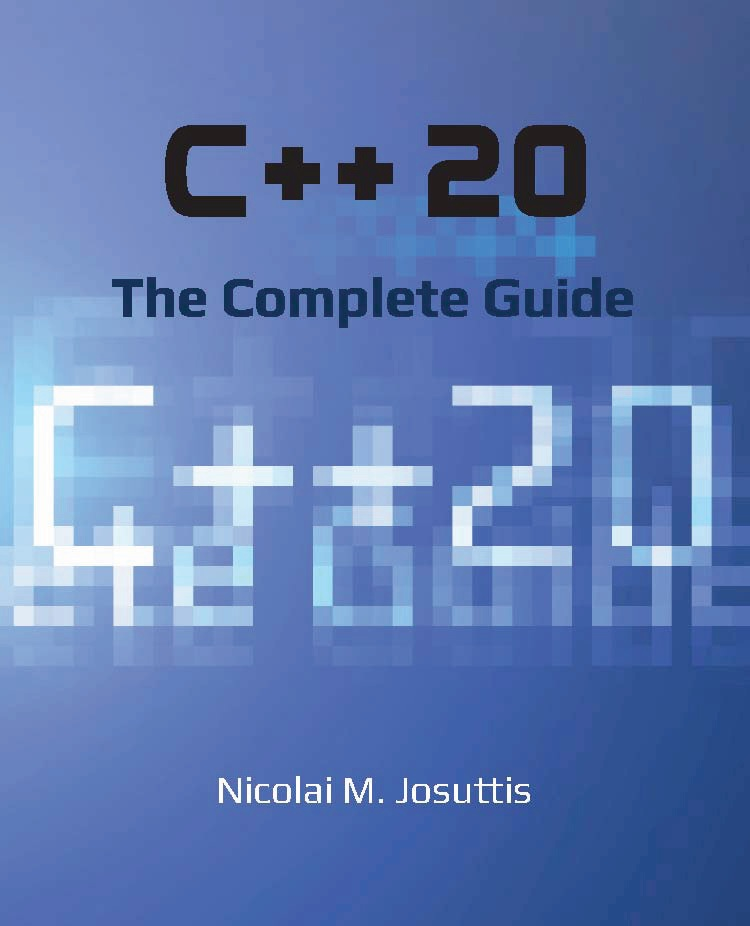
\includegraphics[width=\textwidth,height=\textheight,keepaspectratio]{cover.jpg}
			\begin{tikzpicture}[remember picture, overlay, inner sep=0pt]
				\node at (current page.center) 
				{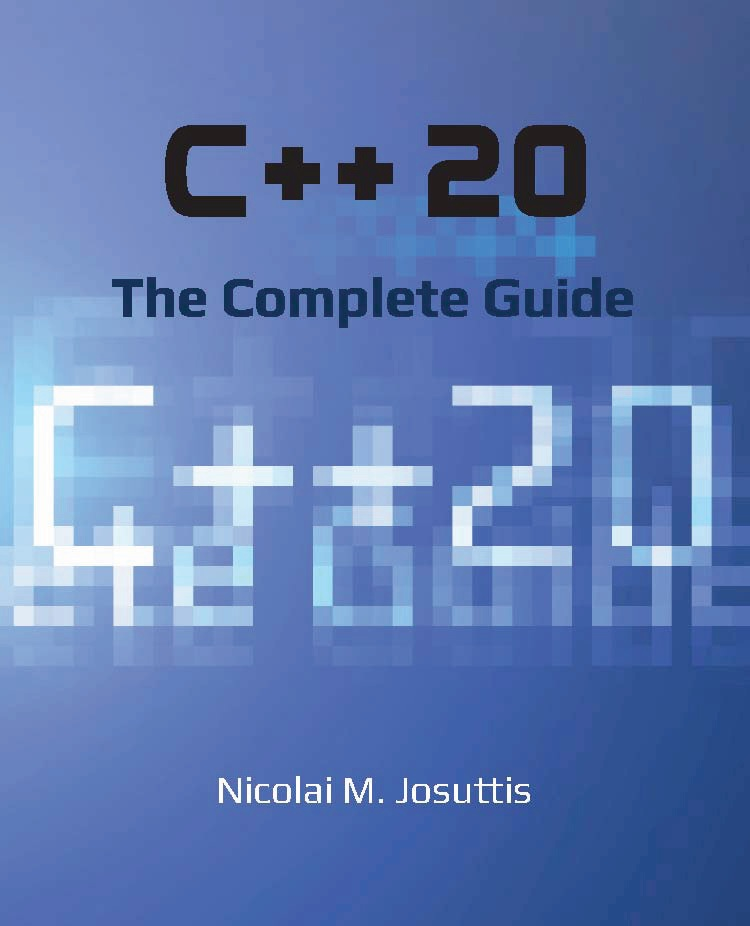
\includegraphics[width=\paperwidth, keepaspectratio=false]{cover.jpg}};
			\end{tikzpicture}
			\newpage
			\thispagestyle{empty}
			\huge
			\textbf{C++20 - The Complete Guide} 
			\\[9pt]
			\normalsize 
			作者: \href{http://www.josuttis.com/welcomee.html}{Nicolai M. Josuttis}
			\\[8pt]
			\normalsize
			译者:\href{https://github.com/xiaoweiChen/CXX20-The-Complete-Guide}{陈晓伟}
			\\[8pt]
			\normalsize 
			版本:\href{http://leanpub.com/cpp20}{2022-10-30}
		\end{center}
		
		\newpage
		
		\pagestyle{empty}		
		\tableofcontents
		\newpage
		
		\setsecnumdepth{section}
		
		\section*{\zihao{2} 前言}
		\addcontentsline{toc}{section}{前言}
		\subfile{content/preface.tex}
		\newpage
		
		\section*{\zihao{2}About This Book}
		\addcontentsline{toc}{section}{About This Book}
		\subfile{content/chapter0/0.tex}
		
		\subsection*{\zihao{3}What You Should Know Before Reading This Book}
		\addcontentsline{toc}{subsection}{What You Should Know Before Reading This Book}
		\subfile{content/chapter0/1.tex}
		
		\subsection*{\zihao{3}Overall Structure of the Book}
		\addcontentsline{toc}{subsection}{Overall Structure of the Book}
		\subfile{content/chapter0/2.tex}
		
		\subsection*{\zihao{3}How to Read This Book}
		\addcontentsline{toc}{subsection}{How to Read This Book}
		\subfile{content/chapter0/3.tex}
		
		\subsection*{\zihao{3}The Way I Implement}
		\addcontentsline{toc}{subsection}{The Way I Implement}
		\subfile{content/chapter0/4.tex}
		
		\subsection*{\zihao{3}The C++ Standards}
		\addcontentsline{toc}{subsection}{The C++ Standards}
		\subfile{content/chapter0/5.tex}
		
		\subsection*{\zihao{3}Example Code and Additional Information}
		\addcontentsline{toc}{subsection}{Example Code and Additional Information}
		\subfile{content/chapter0/6.tex}
		
		\subsection*{\zihao{3}Feedback}
		\addcontentsline{toc}{subsection}{Feedback}
		\subfile{content/chapter0/7.tex}
		\newpage
		
		\section*{\zihao{2} 第1章\hspace{0.5cm}Comparisons and Operator <=>}
		\addcontentsline{toc}{section}{第1章\hspace{0.5cm}Comparisons and Operator <=>}
		\subfile{content/chapter1/0.tex}
		
		\subsection*{\zihao{3} 1.1.\hspace{0.2cm}Motivation for Operator<=>}
		\addcontentsline{toc}{subsection}{1.1.\hspace{0.2cm}Motivation for Operator<=>}
		\subfile{content/chapter1/1.tex}
		
		\subsection*{\zihao{3} 1.2.\hspace{0.2cm}Defining and Using Comparisons}
		\addcontentsline{toc}{subsection}{1.2.\hspace{0.2cm}Defining and Using Comparisons}
		\subfile{content/chapter1/2.tex}
		
		\subsection*{\zihao{3} 1.3.\hspace{0.2cm}Defining operator<=> and operator==}
		\addcontentsline{toc}{subsection}{1.3.\hspace{0.2cm}Defining operator<=> and operator==}
		\subfile{content/chapter1/3.tex}
		
		\subsection*{\zihao{3} 1.4.\hspace{0.2cm}Overload Resolution with Rewritten Expressions}
		\addcontentsline{toc}{subsection}{1.4.\hspace{0.2cm}Overload Resolution with Rewritten Expressions}
		\subfile{content/chapter1/4.tex}
		
		\subsection*{\zihao{3} 1.5.\hspace{0.2cm}Using Operator <=> in Generic Code}
		\addcontentsline{toc}{subsection}{1.5.\hspace{0.2cm}Using Operator <=> in Generic Code}
		\subfile{content/chapter1/5.tex}
		
		\subsection*{\zihao{3} 1.6.\hspace{0.2cm}Compatibility Issues with the Comparison Operators}
		\addcontentsline{toc}{subsection}{1.6.\hspace{0.2cm}Compatibility Issues with the Comparison Operators}
		\subfile{content/chapter1/6.tex}
		
		\subsection*{\zihao{3} 1.7.\hspace{0.2cm}Afternotes}
		\addcontentsline{toc}{subsection}{1.7.\hspace{0.2cm}Afternotes}
		\subfile{content/chapter1/7.tex}
		\newpage
		
		\section*{\zihao{2} 第2章\hspace{0.5cm}Placeholder Types for Function Parameters}
		\addcontentsline{toc}{section}{第2章\hspace{0.5cm}Placeholder Types for Function Parameters}
		\subfile{content/chapter2/0.tex}
		
		\subsection*{\zihao{3} 2.1.\hspace{0.2cm}auto for Parameters of Ordinary Functions}
		\addcontentsline{toc}{subsection}{2.1.\hspace{0.2cm}auto for Parameters of Ordinary Functions}
		\subfile{content/chapter2/1.tex}
		
		\subsection*{\zihao{3} 2.2.\hspace{0.2cm}Using auto for Parameters in Practice}
		\addcontentsline{toc}{subsection}{2.2.\hspace{0.2cm}Using auto for Parameters in Practice}
		\subfile{content/chapter2/2.tex}
		
		\subsection*{\zihao{3} 2.3.\hspace{0.2cm}auto for Parameters in Detail}
		\addcontentsline{toc}{subsection}{2.3.\hspace{0.2cm}auto for Parameters in Detail}
		\subfile{content/chapter2/3.tex}
		
		\subsection*{\zihao{3} 2.4.\hspace{0.2cm}Afternotes}
		\addcontentsline{toc}{subsection}{2.4.\hspace{0.2cm}Afternotes}
		\subfile{content/chapter2/4.tex}
		\newpage
		
		\section*{\zihao{2} 第3章\hspace{0.5cm}Concepts, Requirements, and Constraints}
		\addcontentsline{toc}{section}{第3章\hspace{0.5cm}Concepts, Requirements, and Constraints}
		\subfile{content/chapter3/0.tex}
		
		\subsection*{\zihao{3} 3.1.\hspace{0.2cm}Motivating Example of Concepts and Requirements}
		\addcontentsline{toc}{subsection}{3.1.\hspace{0.2cm}Motivating Example of Concepts and Requirements}
		\subfile{content/chapter3/1.tex}
		
		\subsection*{\zihao{3} 3.2.\hspace{0.2cm}Where Constraints and Concepts Can Be Used}
		\addcontentsline{toc}{subsection}{3.2.\hspace{0.2cm}Where Constraints and Concepts Can Be Used}
		\subfile{content/chapter3/2.tex}
		
		\subsection*{\zihao{3} 3.3.\hspace{0.2cm}Typical Applications of Concepts and Constraints in Practice}
		\addcontentsline{toc}{subsection}{3.3.\hspace{0.2cm}Typical Applications of Concepts and Constraints in Practice}
		\subfile{content/chapter3/3.tex}
		
		\subsection*{\zihao{3} 3.4.\hspace{0.2cm}Semantic Constraints}
		\addcontentsline{toc}{subsection}{3.4.\hspace{0.2cm}Semantic Constraints}
		\subfile{content/chapter3/4.tex}
		
		\subsection*{\zihao{3} 3.5.\hspace{0.2cm}Design Guidelines for Concepts}
		\addcontentsline{toc}{subsection}{3.5.\hspace{0.2cm}Design Guidelines for Concepts}
		\subfile{content/chapter3/5.tex}
		
		\subsection*{\zihao{3} 3.6.\hspace{0.2cm}Afternotes}
		\addcontentsline{toc}{subsection}{3.6.\hspace{0.2cm}Afternotes}
		\subfile{content/chapter3/6.tex}
		\newpage
		
		\section*{\zihao{2} 第4章\hspace{0.5cm}Concepts, Requirements, and Constraints in Detail}
		\addcontentsline{toc}{section}{第4章\hspace{0.5cm}Concepts, Requirements, and Constraints in Detail}
		\subfile{content/chapter4/0.tex}
		
		\subsection*{\zihao{3} 4.1.\hspace{0.2cm}Constraints}
		\addcontentsline{toc}{subsection}{4.1.\hspace{0.2cm}Constraints}
		\subfile{content/chapter4/1.tex}
		
		\subsection*{\zihao{3} 4.2.\hspace{0.2cm}requires Clauses}
		\addcontentsline{toc}{subsection}{4.2.\hspace{0.2cm}requires Clauses}
		\subfile{content/chapter4/2.tex}
		
		\subsection*{\zihao{3} 4.3.\hspace{0.2cm}Ad-hoc Boolean Expressions}
		\addcontentsline{toc}{subsection}{4.3.\hspace{0.2cm}Ad-hoc Boolean Expressions}
		\subfile{content/chapter4/3.tex}
		
		\subsection*{\zihao{3} 4.4.\hspace{0.2cm}requires Expressions}
		\addcontentsline{toc}{subsection}{4.4.\hspace{0.2cm}requires Expressions}
		\subfile{content/chapter4/4.tex}
		
		\subsection*{\zihao{3} 4.5.\hspace{0.2cm}Concepts in Detail}
		\addcontentsline{toc}{subsection}{4.5.\hspace{0.2cm}Concepts in Detail}
		\subfile{content/chapter4/5.tex}
		
		\subsection*{\zihao{3} 4.6.\hspace{0.2cm}Using Concepts as Type Constraints}
		\addcontentsline{toc}{subsection}{4.6.\hspace{0.2cm}Using Concepts as Type Constraints}
		\subfile{content/chapter4/6.tex}
		
		\subsection*{\zihao{3} 4.7.\hspace{0.2cm}Subsuming Constraints with Concepts}
		\addcontentsline{toc}{subsection}{4.7.\hspace{0.2cm}Subsuming Constraints with Concepts}
		\subfile{content/chapter4/7.tex}
		\newpage
		
		\section*{\zihao{2} 第5章\hspace{0.5cm}Standard Concepts in Detail}
		\addcontentsline{toc}{section}{第5章\hspace{0.5cm}Standard Concepts in Detail}
		\subfile{content/chapter5/0.tex}
		
		\subsection*{\zihao{3} 5.1.\hspace{0.2cm}Overview of All Standard Concepts}
		\addcontentsline{toc}{subsection}{5.1.\hspace{0.2cm}Overview of All Standard Concepts}
		\subfile{content/chapter5/1.tex}
		
		\subsection*{\zihao{3} 5.2.\hspace{0.2cm}Language-Related Concepts}
		\addcontentsline{toc}{subsection}{5.2.\hspace{0.2cm}Language-Related Concepts}
		\subfile{content/chapter5/2.tex}
		
		\subsection*{\zihao{3} 5.3.\hspace{0.2cm}Concepts for Iterators and Ranges}
		\addcontentsline{toc}{subsection}{5.3.\hspace{0.2cm}Concepts for Iterators and Ranges}
		\subfile{content/chapter5/3.tex}
		
		\subsection*{\zihao{3} 5.4.\hspace{0.2cm}Concepts for Callables}
		\addcontentsline{toc}{subsection}{5.4.\hspace{0.2cm}Concepts for Callables}
		\subfile{content/chapter5/4.tex}
		
		\subsection*{\zihao{3} 5.5.\hspace{0.2cm}Auxiliary Concepts}
		\addcontentsline{toc}{subsection}{5.5.\hspace{0.2cm}Auxiliary Concepts}
		\subfile{content/chapter5/5.tex}
		\newpage
		
		\section*{\zihao{2} 第6章\hspace{0.5cm}Ranges and Views}
		\addcontentsline{toc}{section}{第6章\hspace{0.5cm}Ranges and Views}
		\subfile{content/chapter6/0.tex}
		
		\subsection*{\zihao{3} 6.1.\hspace{0.2cm}A Tour of Ranges and Views Using Examples}
		\addcontentsline{toc}{subsection}{6.1.\hspace{0.2cm}A Tour of Ranges and Views Using Examples}
		\subfile{content/chapter6/1.tex}
		
		\subsection*{\zihao{3} 6.2.\hspace{0.2cm}Borrowed Iterators and Ranges}
		\addcontentsline{toc}{subsection}{6.2.\hspace{0.2cm}Borrowed Iterators and Ranges}
		\subfile{content/chapter6/2.tex}
		
		\subsection*{\zihao{3} 6.3.\hspace{0.2cm}Using Views}
		\addcontentsline{toc}{subsection}{6.3.\hspace{0.2cm}Using Views}
		\subfile{content/chapter6/3.tex}
		
		\subsection*{\zihao{3} 6.4.\hspace{0.2cm}Views on Ranges That Are Destroyed or Modified}
		\addcontentsline{toc}{subsection}{6.4.\hspace{0.2cm}Views on Ranges That Are Destroyed or Modified}
		\subfile{content/chapter6/4.tex}
		
		\subsection*{\zihao{3} 6.5.\hspace{0.2cm}Views and const}
		\addcontentsline{toc}{subsection}{6.5.\hspace{0.2cm}Views and const}
		\subfile{content/chapter6/5.tex}
		
		\subsection*{\zihao{3} 6.6.\hspace{0.2cm}Summary of All Container Idioms Broken By Views}
		\addcontentsline{toc}{subsection}{6.6.\hspace{0.2cm}Summary of All Container Idioms Broken By Views}
		\subfile{content/chapter6/6.tex}
		
		\subsection*{\zihao{3} 6.7.\hspace{0.2cm}Afternotes}
		\addcontentsline{toc}{subsection}{6.7.\hspace{0.2cm}Afternotes}		\subfile{content/chapter6/7.tex}
		\newpage
		
		\section*{\zihao{2} 第7章\hspace{0.5cm}Utilities for Ranges and Views}
		\addcontentsline{toc}{section}{第7章\hspace{0.5cm}Utilities for Ranges and Views}
		\subfile{content/chapter7/0.tex}
		
		\subsection*{\zihao{3} 7.1.\hspace{0.2cm}Key Utilities for Using Ranges as Views}
		\addcontentsline{toc}{subsection}{7.1.\hspace{0.2cm}Key Utilities for Using Ranges as Views}
		\subfile{content/chapter7/1.tex}
		
		\subsection*{\zihao{3} 7.2.\hspace{0.2cm}New Iterator Categories}
		\addcontentsline{toc}{subsection}{7.2.\hspace{0.2cm}New Iterator Categoriess}
		\subfile{content/chapter7/2.tex}
		
		\subsection*{\zihao{3} 7.3.\hspace{0.2cm}New Iterator and Sentinel Types}
		\addcontentsline{toc}{subsection}{7.3.\hspace{0.2cm}New Iterator and Sentinel Types}
		\subfile{content/chapter7/3.tex}
		
		\subsection*{\zihao{3} 7.4.\hspace{0.2cm}New Functions for Dealing with Ranges}
		\addcontentsline{toc}{subsection}{7.4.\hspace{0.2cm}New Functions for Dealing with Ranges}
		\subfile{content/chapter7/4.tex}
		
		\subsection*{\zihao{3} 7.5.\hspace{0.2cm}New Type Functions/Utilities for Dealing with Ranges}
		\addcontentsline{toc}{subsection}{7.5.\hspace{0.2cm}New Type Functions/Utilities for Dealing with Ranges}
		\subfile{content/chapter7/5.tex}
		
		\subsection*{\zihao{3} 7.6.\hspace{0.2cm}Range Algorithms}
		\addcontentsline{toc}{subsection}{7.6.\hspace{0.2cm}Range Algorithms}
		\subfile{content/chapter7/6.tex}
		\newpage
		
		\section*{\zihao{2} 第8章\hspace{0.5cm}View Types in Detail}
		\addcontentsline{toc}{section}{第8章\hspace{0.5cm}View Types in Details}
		\subfile{content/chapter8/0.tex}
		
		\subsection*{\zihao{3} 8.1.\hspace{0.2cm}Overview of All Views}
		\addcontentsline{toc}{subsection}{8.1.\hspace{0.2cm}Overview of All Views}
		\subfile{content/chapter8/1.tex}
		
		\subsection*{\zihao{3} 8.2.\hspace{0.2cm}Base Class and Namespace of Views}
		\addcontentsline{toc}{subsection}{8.2.\hspace{0.2cm}Base Class and Namespace of Views}
		\subfile{content/chapter8/2.tex}
		
		\subsection*{\zihao{3} 8.3.\hspace{0.2cm}Source Views to External Elements}
		\addcontentsline{toc}{subsection}{8.3.\hspace{0.2cm}Source Views to External Elements}
		\subfile{content/chapter8/3.tex}
		
		\subsection*{\zihao{3} 8.4.\hspace{0.2cm}Generating Views}
		\addcontentsline{toc}{subsection}{8.4.\hspace{0.2cm}Generating Views}
		\subfile{content/chapter8/4.tex}
		
		\subsection*{\zihao{3} 8.5.\hspace{0.2cm}Filtering Views}
		\addcontentsline{toc}{subsection}{8.5.\hspace{0.2cm}Filtering Views}
		\subfile{content/chapter8/5.tex}
		
		\subsection*{\zihao{3} 8.6.\hspace{0.2cm}Transforming Views}
		\addcontentsline{toc}{subsection}{8.6.\hspace{0.2cm}Transforming Views}
		\subfile{content/chapter8/6.tex}
		
		\subsection*{\zihao{3} 8.7.\hspace{0.2cm}Mutating Views}
		\addcontentsline{toc}{subsection}{8.7.\hspace{0.2cm}Mutating Views}
		\subfile{content/chapter8/7.tex}
		
		\subsection*{\zihao{3} 8.8.\hspace{0.2cm}Views for Multiple Ranges}
		\addcontentsline{toc}{subsection}{8.8.\hspace{0.2cm}Views for Multiple Ranges}
		\subfile{content/chapter8/8.tex}
		\newpage
		
		\section*{\zihao{2} 第9章\hspace{0.5cm}Spans}
		\addcontentsline{toc}{section}{第9章\hspace{0.5cm}Spans}
		\subfile{content/chapter9/0.tex}
		
		\subsection*{\zihao{3} 9.1.\hspace{0.2cm}Using Spans}
		\addcontentsline{toc}{subsection}{9.1.\hspace{0.2cm}Using Spans}
		\subfile{content/chapter9/1.tex}
		
		\subsection*{\zihao{3} 9.2.\hspace{0.2cm}Spans Considered Harmful}
		\addcontentsline{toc}{subsection}{9.2.\hspace{0.2cm}Spans Considered Harmful}
		\subfile{content/chapter9/2.tex}
		
		\subsection*{\zihao{3} 9.3.\hspace{0.2cm}Design Aspects of Spans}
		\addcontentsline{toc}{subsection}{9.3.\hspace{0.2cm}Design Aspects of Spans}
		\subfile{content/chapter9/3.tex}
		
		\subsection*{\zihao{3} 9.4.\hspace{0.2cm}Span Operations}
		\addcontentsline{toc}{subsection}{9.4.\hspace{0.2cm}Span Operations}
		\subfile{content/chapter9/4.tex}
		
		\subsection*{\zihao{3} 9.5.\hspace{0.2cm}Afternotes}
		\addcontentsline{toc}{subsection}{9.5.\hspace{0.2cm}Afternotes}
		\subfile{content/chapter9/5.tex}
		\newpage
		
		\section*{\zihao{2} 第10章\hspace{0.5cm}Formatted Output}
		\addcontentsline{toc}{section}{第10章\hspace{0.5cm}Formatted Output}
		\subfile{content/chapter10/0.tex}
		
		\subsection*{\zihao{3} 10.1.\hspace{0.2cm}Formatted Output by Example}
		\addcontentsline{toc}{subsection}{10.1.\hspace{0.2cm}Formatted Output by Example}
		\subfile{content/chapter10/1.tex}
		
		\subsection*{\zihao{3} 10.2.\hspace{0.2cm}Performance of the Formatting Library}
		\addcontentsline{toc}{subsection}{10.2.\hspace{0.2cm}Performance of the Formatting Library}
		\subfile{content/chapter10/2.tex}
		
		\subsection*{\zihao{3} 10.3.\hspace{0.2cm}Formatted Output in Detail}
		\addcontentsline{toc}{subsection}{10.3.\hspace{0.2cm}Formatted Output in Detail}
		\subfile{content/chapter10/3.tex}
		
		\subsection*{\zihao{3} 10.4.\hspace{0.2cm}Internationalization}
		\addcontentsline{toc}{subsection}{10.4.\hspace{0.2cm}Internationalization}
		\subfile{content/chapter10/4.tex}
		
		\subsection*{\zihao{3} 10.5.\hspace{0.2cm}Error Handling}
		\addcontentsline{toc}{subsection}{10.5.\hspace{0.2cm}Error Handling}
		\subfile{content/chapter10/5.tex}
		
		\subsection*{\zihao{3} 10.6.\hspace{0.2cm}User-Defined Formatted Output}
		\addcontentsline{toc}{subsection}{10.6.\hspace{0.2cm}User-Defined Formatted Output}
		\subfile{content/chapter10/6.tex}
		
		\subsection*{\zihao{3} 10.7.\hspace{0.2cm}Afternotes}
		\addcontentsline{toc}{subsection}{10.7.\hspace{0.2cm}Afternotes}
		\subfile{content/chapter10/7.tex}
		\newpage
		
		\section*{\zihao{2} 第11章\hspace{0.5cm}Dates and Timezones for <chrono>}
		\addcontentsline{toc}{section}{第11章\hspace{0.5cm}Dates and Timezones for <chrono>}
		\subfile{content/chapter11/0.tex}
		
		\subsection*{\zihao{3} 11.1.\hspace{0.2cm}Overview by Example}
		\addcontentsline{toc}{subsection}{11.1.\hspace{0.2cm}Overview by Example}
		\subfile{content/chapter11/1.tex}
		
		\subsection*{\zihao{3} 11.2.\hspace{0.2cm}Basic Chrono Concepts and Terminology}
		\addcontentsline{toc}{subsection}{11.2.\hspace{0.2cm}Basic Chrono Concepts and Terminology}
		\subfile{content/chapter11/2.tex}
		
		\subsection*{\zihao{3} 11.3.\hspace{0.2cm}Basic Chrono Extensions with C++20}
		\addcontentsline{toc}{subsection}{11.3.\hspace{0.2cm}Basic Chrono Extensions with C++20}
		\subfile{content/chapter11/3.tex}
		
		\subsection*{\zihao{3} 11.4.\hspace{0.2cm}I/O with Chrono Types}
		\addcontentsline{toc}{subsection}{11.4.\hspace{0.2cm}I/O with Chrono Types}
		\subfile{content/chapter11/4.tex}
		
		\subsection*{\zihao{3} 11.5.\hspace{0.2cm}Using the Chrono Extensions in Practice}
		\addcontentsline{toc}{subsection}{11.5.\hspace{0.2cm}Using the Chrono Extensions in Practice}
		\subfile{content/chapter11/5.tex}
		
		\subsection*{\zihao{3} 11.6.\hspace{0.2cm}Timezones}
		\addcontentsline{toc}{subsection}{11.6.\hspace{0.2cm}Timezones}
		\subfile{content/chapter11/6.tex}
		
		\subsection*{\zihao{3} 11.7.\hspace{0.2cm}Clocks in Detail}
		\addcontentsline{toc}{subsection}{11.7.\hspace{0.2cm}Clocks in Detail}
		\subfile{content/chapter11/7.tex}
		
		\subsection*{\zihao{3} 11.8.\hspace{0.2cm}Other New Chrono Features}
		\addcontentsline{toc}{subsection}{11.8.\hspace{0.2cm}Other New Chrono Features}
		\subfile{content/chapter11/8.tex}
		
		\subsection*{\zihao{3} 11.9.\hspace{0.2cm}Afternotes}
		\addcontentsline{toc}{subsection}{11.9.\hspace{0.2cm}Afternotes}
		\subfile{content/chapter11/9.tex}
		\newpage
		
		\section*{\zihao{2} 第12章\hspace{0.5cm}std::jthread and Stop Tokens}
		\addcontentsline{toc}{section}{第12章\hspace{0.5cm}std::jthread and Stop Tokens}
		\subfile{content/chapter12/0.tex}
		
		\subsection*{\zihao{3} 12.1.\hspace{0.2cm}Motivation for std::jthread}
		\addcontentsline{toc}{subsection}{12.1.\hspace{0.2cm}Motivation for std::jthread}
		\subfile{content/chapter12/1.tex}
		
		\subsection*{\zihao{3} 12.2.\hspace{0.2cm}Stop Sources and Stop Tokens}
		\addcontentsline{toc}{subsection}{12.2.\hspace{0.2cm}Stop Sources and Stop Tokens}
		\subfile{content/chapter12/2.tex}
		
		\subsection*{\zihao{3} 12.3.\hspace{0.2cm}std::jthread in Detail}
		\addcontentsline{toc}{subsection}{12.3.\hspace{0.2cm}std::jthread in Detail}
		\subfile{content/chapter12/3.tex}
		
		\subsection*{\zihao{3} 12.4.\hspace{0.2cm}Afternotes}
		\addcontentsline{toc}{subsection}{12.4.\hspace{0.2cm}Afternotes}
		\subfile{content/chapter12/4.tex}
		\newpage
		
		\section*{\zihao{2} 第13章\hspace{0.5cm}Concurrency Features}
		\addcontentsline{toc}{section}{第13章\hspace{0.5cm}Concurrency Features}
		\subfile{content/chapter13/0.tex}
		
		\subsection*{\zihao{3} 13.1.\hspace{0.2cm}Thread Synchronization with Latches and Barriers}
		\addcontentsline{toc}{subsection}{13.1.\hspace{0.2cm}Thread Synchronization with Latches and Barriers}
		\subfile{content/chapter13/1.tex}
		
		\subsection*{\zihao{3} 13.2.\hspace{0.2cm}Semaphores}
		\addcontentsline{toc}{subsection}{13.2.\hspace{0.2cm}Semaphores}
		\subfile{content/chapter13/2.tex}
		
		\subsection*{\zihao{3} 13.3.\hspace{0.2cm}Extensions for Atomic Types}
		\addcontentsline{toc}{subsection}{13.3.\hspace{0.2cm}Extensions for Atomic Types}
		\subfile{content/chapter13/3.tex}
		
		\subsection*{\zihao{3} 13.4.\hspace{0.2cm}Synchronized Output Streams}
		\addcontentsline{toc}{subsection}{13.4.\hspace{0.2cm}Synchronized Output Streams}
		\subfile{content/chapter13/4.tex}
		
		\subsection*{\zihao{3} 13.5.\hspace{0.2cm}Afternotes}
		\addcontentsline{toc}{subsection}{13.5.\hspace{0.2cm}Afternotes}
		\subfile{content/chapter13/5.tex}
		\newpage
		
		\section*{\zihao{2} 第14章\hspace{0.5cm}Coroutines}
		\addcontentsline{toc}{section}{第14章\hspace{0.5cm}Coroutines}
		\subfile{content/chapter14/0.tex}
		
		\subsection*{\zihao{3} 14.1.\hspace{0.2cm}What Are Coroutines?}
		\addcontentsline{toc}{subsection}{14.1.\hspace{0.2cm}What Are Coroutines?}
		\subfile{content/chapter14/1.tex}
		
		\subsection*{\zihao{3} 14.2.\hspace{0.2cm}A First Coroutine Example}
		\addcontentsline{toc}{subsection}{14.2.\hspace{0.2cm}A First Coroutine Example}
		\subfile{content/chapter14/2.tex}
		
		\subsection*{\zihao{3} 14.3.\hspace{0.2cm}Coroutines That Yield or Return Values}
		\addcontentsline{toc}{subsection}{14.3.\hspace{0.2cm}Coroutines That Yield or Return Values}
		\subfile{content/chapter14/3.tex}
		
		\subsection*{\zihao{3} 14.4.\hspace{0.2cm}Coroutine Awaitables and Awaiters}
		\addcontentsline{toc}{subsection}{14.4.\hspace{0.2cm}Coroutine Awaitables and Awaiters}
		\subfile{content/chapter14/4.tex}
		
		\subsection*{\zihao{3} 14.5.\hspace{0.2cm}Afternotes}
		\addcontentsline{toc}{subsection}{14.5.\hspace{0.2cm}Afternotes}
		\subfile{content/chapter14/5.tex}
		\newpage
		
		\section*{\zihao{2} 第15章\hspace{0.5cm}Coroutines in Detail}
		\addcontentsline{toc}{section}{第15章\hspace{0.5cm}Coroutines in Detail}
		\subfile{content/chapter15/0.tex}
		
		\subsection*{\zihao{3} 15.1.\hspace{0.2cm}Coroutine Constraints}
		\addcontentsline{toc}{subsection}{15.1.\hspace{0.2cm}Coroutine Constraints}
		\subfile{content/chapter15/1.tex}
		
		\subsection*{\zihao{3} 15.2.\hspace{0.2cm}The Coroutine Frame and the Promises}
		\addcontentsline{toc}{subsection}{15.2.\hspace{0.2cm}The Coroutine Frame and the Promises}
		\subfile{content/chapter15/2.tex}
		
		\subsection*{\zihao{3} 15.3.\hspace{0.2cm}Coroutine Promises in Detail}
		\addcontentsline{toc}{subsection}{15.3.\hspace{0.2cm}Coroutine Promises in Detail}
		\subfile{content/chapter15/3.tex}
		
		\subsection*{\zihao{3} 15.4.\hspace{0.2cm}Coroutine Handles in Detail}
		\addcontentsline{toc}{subsection}{15.4.\hspace{0.2cm}Coroutine Handles in Detail}
		\subfile{content/chapter15/4.tex}
		
		\subsection*{\zihao{3} 15.5.\hspace{0.2cm}Exceptions in Coroutines}
		\addcontentsline{toc}{subsection}{15.5.\hspace{0.2cm}Exceptions in Coroutines}
		\subfile{content/chapter15/5.tex}
		
		\subsection*{\zihao{3} 15.6.\hspace{0.2cm}Allocating Memory for the Coroutine Frame}
		\addcontentsline{toc}{subsection}{15.6.\hspace{0.2cm}Allocating Memory for the Coroutine Frame}
		\subfile{content/chapter15/6.tex}
		
		\subsection*{\zihao{3} 15.7.\hspace{0.2cm}co\_await and Awaiters in Detail}
		\addcontentsline{toc}{subsection}{15.7.\hspace{0.2cm}co\_await and Awaiters in Detail}
		\subfile{content/chapter15/7.tex}
		
		\subsection*{\zihao{3} 15.8.\hspace{0.2cm}Other Ways of Dealing with co\_await}
		\addcontentsline{toc}{subsection}{15.8.\hspace{0.2cm}Other Ways of Dealing with co\_await}
		\subfile{content/chapter15/8.tex}
		
		\subsection*{\zihao{3} 15.9.\hspace{0.2cm}Concurrent Use of Coroutines}
		\addcontentsline{toc}{subsection}{15.9.\hspace{0.2cm}Concurrent Use of Coroutines}
		\subfile{content/chapter15/9.tex}
		
		\subsection*{\zihao{3} 15.10.\hspace{0.2cm}Coroutine Traits}
		\addcontentsline{toc}{subsection}{15.10.\hspace{0.2cm}Coroutine Traits}
		\subfile{content/chapter15/10.tex}
		\newpage
		
		\section*{\zihao{2} 第16章\hspace{0.5cm}Modules}
		\addcontentsline{toc}{section}{第16章\hspace{0.5cm}Modules}
		\subfile{content/chapter16/0.tex}
		
		\subsection*{\zihao{3} 16.1.\hspace{0.2cm}Motivation for Modules Using a First Example}
		\addcontentsline{toc}{subsection}{16.1.\hspace{0.2cm}Motivation for Modules Using a First Example}
		\subfile{content/chapter16/1.tex}
		
		\subsection*{\zihao{3} 16.2.\hspace{0.2cm}Modules with Multiple Files}
		\addcontentsline{toc}{subsection}{16.2.\hspace{0.2cm}Modules with Multiple Files}
		\subfile{content/chapter16/2.tex}
		
		\subsection*{\zihao{3} 16.3.\hspace{0.2cm}Dealing with Modules in Practice}
		\addcontentsline{toc}{subsection}{16.3.\hspace{0.2cm}Dealing with Modules in Practice}
		\subfile{content/chapter16/3.tex}
		
		\subsection*{\zihao{3} 16.4.\hspace{0.2cm}Modules in Detail}
		\addcontentsline{toc}{subsection}{16.4.\hspace{0.2cm}Modules in Detail}
		\subfile{content/chapter16/4.tex}
		
		\subsection*{\zihao{3} 16.5.\hspace{0.2cm}Afternotes}
		\addcontentsline{toc}{subsection}{16.5.\hspace{0.2cm}Afternotes}
		\subfile{content/chapter16/5.tex}
		\newpage
		
		\section*{\zihao{2} 第17章\hspace{0.5cm}Lambda Extensions}
		\addcontentsline{toc}{section}{第17章\hspace{0.5cm}Lambda Extensions}
		\subfile{content/chapter17/0.tex}
		
		\subsection*{\zihao{3} 17.1.\hspace{0.2cm}Generic Lambdas with Template Parameters}
		\addcontentsline{toc}{subsection}{17.1.\hspace{0.2cm}Generic Lambdas with Template Parameters}
		\subfile{content/chapter17/1.tex}
		
		\subsection*{\zihao{3} 17.2.\hspace{0.2cm}Calling the Default Constructor of Lambdas}
		\addcontentsline{toc}{subsection}{17.2.\hspace{0.2cm}Calling the Default Constructor of Lambdas}
		\subfile{content/chapter17/2.tex}
		
		\subsection*{\zihao{3} 17.3.\hspace{0.2cm}Lambdas as Non-Type Template Parameters}
		\addcontentsline{toc}{subsection}{17.3.\hspace{0.2cm}Lambdas as Non-Type Template Parameters}
		\subfile{content/chapter17/3.tex}
		
		\subsection*{\zihao{3} 17.4.\hspace{0.2cm}consteval Lambdas}
		\addcontentsline{toc}{subsection}{17.4.\hspace{0.2cm}consteval Lambdas}
		\subfile{content/chapter17/4.tex}
		
		\subsection*{\zihao{3} 17.5.\hspace{0.2cm}Changes for Capturing}
		\addcontentsline{toc}{subsection}{17.5.\hspace{0.2cm}Changes for Capturing}
		\subfile{content/chapter17/5.tex}
		
		\subsection*{\zihao{3} 17.6.\hspace{0.2cm}Afternotes}
		\addcontentsline{toc}{subsection}{17.6.\hspace{0.2cm}Afternotes}
		\subfile{content/chapter17/6.tex}
		\newpage
		
		\section*{\zihao{2} 第18章\hspace{0.5cm}Compile-Time Computing}
		\addcontentsline{toc}{section}{第18章\hspace{0.5cm}Compile-Time Computing}
		\subfile{content/chapter17/0.tex}
		
		\subsection*{\zihao{3} 18.1.\hspace{0.2cm}Keyword constinit}
		\addcontentsline{toc}{subsection}{18.1.\hspace{0.2cm}Keyword constinit}
		\subfile{content/chapter18/1.tex}
		
		\subsection*{\zihao{3} 18.2.\hspace{0.2cm}Keyword consteval}
		\addcontentsline{toc}{subsection}{18.2.\hspace{0.2cm}Keyword consteval}
		\subfile{content/chapter18/2.tex}
		
		\subsection*{\zihao{3} 18.3.\hspace{0.2cm}Relaxed Constraints for constexpr Functions}
		\addcontentsline{toc}{subsection}{18.3.\hspace{0.2cm}Relaxed Constraints for constexpr Functions}
		\subfile{content/chapter18/3.tex}
		
		\subsection*{\zihao{3} 18.4.\hspace{0.2cm}std::is\_constant\_evaluated()}
		\addcontentsline{toc}{subsection}{18.4.\hspace{0.2cm}std::is\_constant\_evaluated()}
		\subfile{content/chapter18/4.tex}
		
		\subsection*{\zihao{3} 18.5.\hspace{0.2cm}Using Heap Memory, Vectors, and Strings at Compile Time}
		\addcontentsline{toc}{subsection}{18.5.\hspace{0.2cm}Using Heap Memory, Vectors, and Strings at Compile Time}
		\subfile{content/chapter18/5.tex}
		
		\subsection*{\zihao{3} 18.6.\hspace{0.2cm}Other constexpr Extensions}
		\addcontentsline{toc}{subsection}{18.6.\hspace{0.2cm}Other constexpr Extensions}
		\subfile{content/chapter18/6.tex}
		
		\subsection*{\zihao{3} 18.7.\hspace{0.2cm}Afternotes}
		\addcontentsline{toc}{subsection}{18.7.\hspace{0.2cm}Afternotes}
		\subfile{content/chapter18/7.tex}
		\newpage
		
		\section*{\zihao{2} 第19章\hspace{0.5cm}Non-Type Template Parameter (NTTP) Extensions}
		\addcontentsline{toc}{section}{第19章\hspace{0.5cm}Non-Type Template Parameter (NTTP) Extensions}
		\subfile{content/chapter19/0.tex}
		
		\subsection*{\zihao{3} 19.1.\hspace{0.2cm}New Types for Non-Type Template Parameters}
		\addcontentsline{toc}{subsection}{19.1.\hspace{0.2cm}New Types for Non-Type Template Parameters}
		\subfile{content/chapter19/1.tex}
		
		\subsection*{\zihao{3} 19.2.\hspace{0.2cm}Afternotes}
		\addcontentsline{toc}{subsection}{19.2.\hspace{0.2cm}Afternotes}
		\subfile{content/chapter19/2.tex}
		\newpage
		
		\section*{\zihao{2} 第20章\hspace{0.5cm}New Type Traits}
		\addcontentsline{toc}{section}{第20章\hspace{0.5cm}New Type Traits}
		\subfile{content/chapter20/0.tex}
		
		\subsection*{\zihao{3} 20.1.\hspace{0.2cm}New Type Traits for Type Classification}
		\addcontentsline{toc}{subsection}{20.1.\hspace{0.2cm}New Type Traits for Type Classification}
		\subfile{content/chapter20/1.tex}
		
		\subsection*{\zihao{3} 20.2.\hspace{0.2cm}New Type Traits for Type Inspection}
		\addcontentsline{toc}{subsection}{20.2.\hspace{0.2cm}New Type Traits for Type Inspection}
		\subfile{content/chapter20/2.tex}
		
		\subsection*{\zihao{3} 20.3.\hspace{0.2cm}New Type Traits for Type Conversion}
		\addcontentsline{toc}{subsection}{20.3.\hspace{0.2cm}New Type Traits for Type Conversion}
		\subfile{content/chapter20/3.tex}
		
		\subsection*{\zihao{3} 20.4.\hspace{0.2cm}New Type Traits for Iterators}
		\addcontentsline{toc}{subsection}{20.4.\hspace{0.2cm}New Type Traits for Iterators}
		\subfile{content/chapter20/4.tex}
		
		\subsection*{\zihao{3} 20.5.\hspace{0.2cm}Type Traits and Functions for Layout Compatibility}
		\addcontentsline{toc}{subsection}{20.5.\hspace{0.2cm}Type Traits and Functions for Layout Compatibility}
		\subfile{content/chapter20/5.tex}
		
		\subsection*{\zihao{3} 20.6.\hspace{0.2cm}Afternotes}
		\addcontentsline{toc}{subsection}{20.6.\hspace{0.2cm}Afternotes}
		\subfile{content/chapter20/6.tex}
		\newpage
		
		\section*{\zihao{2} 第21章\hspace{0.5cm}Small Improvements for the Core Language}
		\addcontentsline{toc}{section}{第21章\hspace{0.5cm}Small Improvements for the Core Language}
		\subfile{content/chapter21/0.tex}
		
		\subsection*{\zihao{3} 21.1.\hspace{0.2cm}Range-Based for Loop with Initialization}
		\addcontentsline{toc}{subsection}{21.1.\hspace{0.2cm}Range-Based for Loop with Initialization}
		\subfile{content/chapter21/1.tex}
		
		\subsection*{\zihao{3} 21.2.\hspace{0.2cm}using for Enumeration Values}
		\addcontentsline{toc}{subsection}{21.2.\hspace{0.2cm}using for Enumeration Values}
		\subfile{content/chapter21/2.tex}
		
		\subsection*{\zihao{3} 21.3.\hspace{0.2cm}Delegating Enumeration Types to Different Scopes}
		\addcontentsline{toc}{subsection}{21.3.\hspace{0.2cm}Delegating Enumeration Types to Different Scopes}
		\subfile{content/chapter21/3.tex}
		
		\subsection*{\zihao{3} 21.4.\hspace{0.2cm}New Character Type char8\_t}
		\addcontentsline{toc}{subsection}{21.4.\hspace{0.2cm}New Character Type char8\_t}
		\subfile{content/chapter21/4.tex}
		
		\subsection*{\zihao{3} 21.5.\hspace{0.2cm}Improvements for Aggregates}
		\addcontentsline{toc}{subsection}{21.5.\hspace{0.2cm}Improvements for Aggregates}
		\subfile{content/chapter21/5.tex}
		
		\subsection*{\zihao{3} 21.6.\hspace{0.2cm}New Attributes and Attribute Features}
		\addcontentsline{toc}{subsection}{21.6.\hspace{0.2cm}New Attributes and Attribute Features}
		\subfile{content/chapter21/6.tex}
		
		\subsection*{\zihao{3} 21.7.\hspace{0.2cm}Feature Test Macros}
		\addcontentsline{toc}{subsection}{21.7.\hspace{0.2cm}Feature Test Macros}
		\subfile{content/chapter21/7.tex}
		
		\subsection*{\zihao{3} 21.8.\hspace{0.2cm}Afternotes}
		\addcontentsline{toc}{subsection}{21.8.\hspace{0.2cm}Afternotes}
		\subfile{content/chapter21/8.tex}
		\newpage
		
		\section*{\zihao{2} 第22章\hspace{0.5cm}Small Improvements for Generic Programming}
		\addcontentsline{toc}{section}{第22章\hspace{0.5cm}Small Improvements for Generic Programming}
		\subfile{content/chapter22/0.tex}
		
		\subsection*{\zihao{3} 22.1.\hspace{0.2cm}Implicit typename for Type Members of Template Parameters}
		\addcontentsline{toc}{subsection}{22.1.\hspace{0.2cm}Implicit typename for Type Members of Template Parameters}
		\subfile{content/chapter22/1.tex}
		
		\subsection*{\zihao{3} 22.2.\hspace{0.2cm}Improvements for Aggregates in Generic Code}
		\addcontentsline{toc}{subsection}{22.2.\hspace{0.2cm}Improvements for Aggregates in Generic Code}
		\subfile{content/chapter22/2.tex}
		
		\subsection*{\zihao{3} 22.3.\hspace{0.2cm}Conditional explicit}
		\addcontentsline{toc}{subsection}{22.3.\hspace{0.2cm}Conditional explicit}
		\subfile{content/chapter22/3.tex}
		
		\subsection*{\zihao{3} 22.4.\hspace{0.2cm}Afternotes}
		\addcontentsline{toc}{subsection}{22.4.\hspace{0.2cm}Afternotes}
		\subfile{content/chapter22/4.tex}
		\newpage
		
		\section*{\zihao{2} 第23章\hspace{0.5cm}Small Improvements for the C++ Standard Library}
		\addcontentsline{toc}{section}{第23章\hspace{0.5cm}Small Improvements for the C++ Standard Library}
		\subfile{content/chapter23/0.tex}
		
		\subsection*{\zihao{3} 23.1.\hspace{0.2cm}Updates for String Types}
		\addcontentsline{toc}{subsection}{23.1.\hspace{0.2cm}Updates for String Typesn}
		\subfile{content/chapter23/1.tex}
		
		\subsection*{\zihao{3} 23.2.\hspace{0.2cm}std::source\_location}
		\addcontentsline{toc}{subsection}{23.2.\hspace{0.2cm}std::source\_location}
		\subfile{content/chapter23/2.tex}
		
		\subsection*{\zihao{3} 23.3.\hspace{0.2cm}Safe Comparisons of Integral Values and Sizes}
		\addcontentsline{toc}{subsection}{23.3.\hspace{0.2cm}Safe Comparisons of Integral Values and Sizes}
		\subfile{content/chapter23/3.tex}
		
		\subsection*{\zihao{3} 23.4.\hspace{0.2cm}Mathematical Constants}
		\addcontentsline{toc}{subsection}{23.4.\hspace{0.2cm}Mathematical Constants}
		\subfile{content/chapter23/4.tex}
		
		\subsection*{\zihao{3} 23.5.\hspace{0.2cm}Utilities for Dealing with Bits}
		\addcontentsline{toc}{subsection}{23.5.\hspace{0.2cm}Utilities for Dealing with Bits}
		\subfile{content/chapter23/5.tex}
		
		\subsection*{\zihao{3} 23.6.\hspace{0.2cm}<version>}
		\addcontentsline{toc}{subsection}{23.6.\hspace{0.2cm}<version>}
		\subfile{content/chapter23/6.tex}
		
		\subsection*{\zihao{3} 23.7.\hspace{0.2cm}Extensions for Algorithms}
		\addcontentsline{toc}{subsection}{23.7.\hspace{0.2cm}Extensions for Algorithms}
		\subfile{content/chapter23/7.tex}
		
		\subsection*{\zihao{3} 23.8.\hspace{0.2cm}Afternotes}
		\addcontentsline{toc}{subsection}{23.8.\hspace{0.2cm}Afternotes}
		\subfile{content/chapter23/8.tex}
		\newpage
		
		\section*{\zihao{2} 第24章\hspace{0.5cm}Deprecated and Removed Features}
		\addcontentsline{toc}{section}{第24章\hspace{0.5cm}Deprecated and Removed Features}
		\subfile{content/chapter24/0.tex}
		
		\subsection*{\zihao{3} 24.1.\hspace{0.2cm}Deprecated and Removed Core Language Features}
		\addcontentsline{toc}{subsection}{24.1.\hspace{0.2cm}Deprecated and Removed Core Language Features}
		\subfile{content/chapter24/1.tex}
		
		\subsection*{\zihao{3} 24.2.\hspace{0.2cm}Deprecated and Removed Library Features}
		\addcontentsline{toc}{subsection}{24.2.\hspace{0.2cm}Deprecated and Removed Library Features}
		\subfile{content/chapter24/2.tex}
		
		\subsection*{\zihao{3} 24.3.\hspace{0.2cm}Afternotes}
		\addcontentsline{toc}{subsection}{24.3.\hspace{0.2cm}Afternotes}
		\subfile{content/chapter24/3.tex}
		\newpage
		
		\section*{\zihao{2} Glossary}
		\addcontentsline{toc}{section}{Glossary}
		\subfile{content/chapter25/0.tex}
		
		\subsection*{\zihao{3} A}
		\addcontentsline{toc}{subsection}{A}
		\subfile{content/chapter25/1.tex}
		
		\subsection*{\zihao{3} C}
		\addcontentsline{toc}{subsection}{C}
		\subfile{content/chapter25/2.tex}
		
		\subsection*{\zihao{3} F}
		\addcontentsline{toc}{subsection}{F}
		\subfile{content/chapter25/3.tex}
		
		\subsection*{\zihao{3} G}
		\addcontentsline{toc}{subsection}{G}
		\subfile{content/chapter23/4.tex}
		
		\subsection*{\zihao{3} I}
		\addcontentsline{toc}{subsection}{I}
		\subfile{content/chapter25/5.tex}
		
		\subsection*{\zihao{3} L}
		\addcontentsline{toc}{subsection}{L}
		\subfile{content/chapter25/6.tex}
		
		\subsection*{\zihao{3} P}
		\addcontentsline{toc}{subsection}{P}
		\subfile{content/chapter25/7.tex}
		
		\subsection*{\zihao{3} R}
		\addcontentsline{toc}{subsection}{R}
		\subfile{content/chapter25/8.tex}
		
		\subsection*{\zihao{3} S}
		\addcontentsline{toc}{subsection}{S}
		\subfile{content/chapter25/9.tex}
		
		\subsection*{\zihao{3} U}
		\addcontentsline{toc}{subsection}{U}
		\subfile{content/chapter25/10.tex}
		
		\subsection*{\zihao{3} V}
		\addcontentsline{toc}{subsection}{V}
		\subfile{content/chapter25/11.tex}
		
		\subsection*{\zihao{3} X}
		\addcontentsline{toc}{subsection}{X}
		\subfile{content/chapter25/12.tex}
		\newpage
		
	\end{sloppypar}
\end{document}

